
% This LaTeX was auto-generated from MATLAB code.
% To make changes, update the MATLAB code and republish this document.

\documentclass{article}
\usepackage{graphicx}
\usepackage{color}

\sloppy
\definecolor{lightgray}{gray}{0.5}
\setlength{\parindent}{0pt}

\begin{document}

    
    
\subsection*{Contents}

\begin{itemize} 
\setlength{\itemsep}{-1ex}
   \item Problem 2
   \item Problem 4
   \item Problem 6
\end{itemize}
\begin{verbatim}
% HW2 ECI 144 Due Jan 30th, 2019
\end{verbatim}


\subsection*{Problem 2}

\begin{verbatim}
clc, clear

SandNum=12;

% Sand 1

q1 = [0.624,1.33,2.08,2.47,2.63,3.78,4.06,4.24,4.82,5.09]; % Specific Discharge (mm/s)

H1i= [1.11,2.36,4,4.9,5.01,7.63,8.13,8.58,9.86,10.89]; % Inlet Head (m)

H1o = zeros(1,length(H1i)); % Outlet Head (m)

delta_h1_dl=-1*(H1o-H1i)./0.58;

tbl1 = table(delta_h1_dl',q1','VariableNames',{'minus_gradient','q'});

lm1 = fitlm(tbl1,'linear','Intercept',false);

x=[0:0.1:19];

fit=lm1.Coefficients{1,1}.*x;






% Sand 2

q2 = [3.26,3.17,3.12,3.01,3.14,2.58,2.1,1.7,1.37,1.5,0.78,0.719]; % Specific Discharge (mm/s)

H2i = [9.48,12.88,9.8,12.87,12.8,8.86,12.84,6.71,12.81,5.58,2.98,12.86]; % Inlet Head (m)

H2o = [-3.6,0,-2.78,0.46,0.49,-0.83,4.4,0,7.03,0,0,9.88]; % Outlet Head (m)

delta_h2_dl=-1*(H2o-H2i)./1.1;

tbl2 = table(delta_h2_dl',q2','VariableNames',{'minus_gradient','q'});

lm2 = fitlm(tbl2,'linear','Intercept',false);

x2=[0:0.1:12];

fit2=lm2.Coefficients{1,1}.*x2;


hold on



    plot(delta_h1_dl,q1, 'kv')
    plot(delta_h2_dl,q2, 'k+')

    plot(x2,fit2,'k--')
    plot(x,fit,'k--')

    text(3.3,4,'y_1=0.2850x, R_1^2=0.9933')
    text(9,2,'y_2=0.2753x, R_2^2=0.9943')



    legend('Sand 2','Linear Model', 'location','NW')

    legend('Sand 1','Sand 2')


xlabel('$\frac{-dH}{dl}$', 'Interpreter','latex','FontSize',20)


ylabel('Specific Discharge (mm/s)', 'Interpreter','latex','FontSize',15)

ax = gca;

% c = ax.Color;
% ax.Color = 'blue';
%
% ax.FontSize = 14
\end{verbatim}

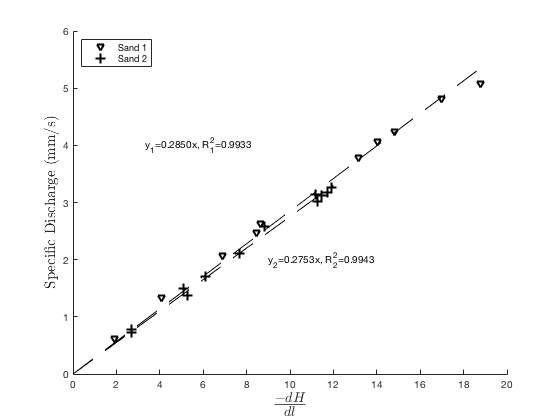
\includegraphics [width=4in]{HomeworkTwo_01.eps}


\subsection*{Problem 4}

\begin{verbatim}
clear,clc
data=[4.3e-4, 6.1e-3, 2.5e-5, 1.2e-4, 1.0e-6, 7.1e-3, 9.1e-6, 2.2e-3, 4.2e-5,8.7e-4, 3.5e-5];

mean(data)
geomean(data)
harmmean(data)
\end{verbatim}

        \color{lightgray} \begin{verbatim}ans =
    0.0015
ans =
   1.5702e-04
ans =
   9.0547e-06
\end{verbatim} \color{black}
    

\subsection*{Problem 6}

\begin{verbatim}
clear,clc

ss = [4.75, 2, 0.84, 0.425, 0.25, 0.106, 0.0750, 0.045, 0.011];  % in mm
mass_retained_sample_A = [49.9, 36.5, 42.1, 40, 23, 11, 10.2, 5, 3];     % g
mrsA=mass_retained_sample_A;
mass_retained_sample_B = [9.9, 46.5, 52.1, 86.2, 80, 25.3, 20.2, 10, 1]; % g
mrsB=mass_retained_sample_B;
mass_retained_sample_C = [16.6, 88, 207, 35.2, 8.3, 3, 0.5, 0.2, 0.1];   % g
mrsC=mass_retained_sample_C;

for k=2:length(mass_retained_sample_A)

    mrsA(k)=mrsA(k-1)+mass_retained_sample_A(k);
    mrsB(k)=mrsB(k-1)+mass_retained_sample_B(k);
    mrsC(k)=mrsC(k-1)+mass_retained_sample_C(k);
end

percent_finerA = 1 - mrsA/sum(mass_retained_sample_A);
percent_finerB = 1 - mrsB/sum(mass_retained_sample_B)
percent_finerC = 1 - mrsC/sum(mass_retained_sample_C);

%cA=polyfit(fliplr(ss), fliplr(percent_finerA),2);

%x=[0:.01:5];

%funA=cA(1).*x.^3+cA(2).*x.^2+cA(3).*x+cA(4);
%funA=cA(1).*x.^2+cA(2).*x.^1+cA(3);
hold on

semilogx(fliplr(ss),fliplr(percent_finerA),'kv-')
semilogx(fliplr(ss),fliplr(percent_finerB),'k+-')
semilogx(fliplr(ss),fliplr(percent_finerC),'ks-')


%semilogx(x,funA,'k-')
set(gca, 'XDir','reverse','GridAlpha',1,'MinorGridAlpha',1)
set(gca,'minorgridlinestyle','-')
set(gca, 'XScale', 'log');
grid on
xlabel('Grain Size (mm)')
ylabel('Percent Finer by Weight')

legend('Sand A','Sand B','Sand C')
\end{verbatim}

        \color{lightgray} \begin{verbatim}percent_finerB =
  Columns 1 through 7
    0.9701    0.8297    0.6724    0.4121    0.1706    0.0942    0.0332
  Columns 8 through 9
    0.0030         0
\end{verbatim} \color{black}
    
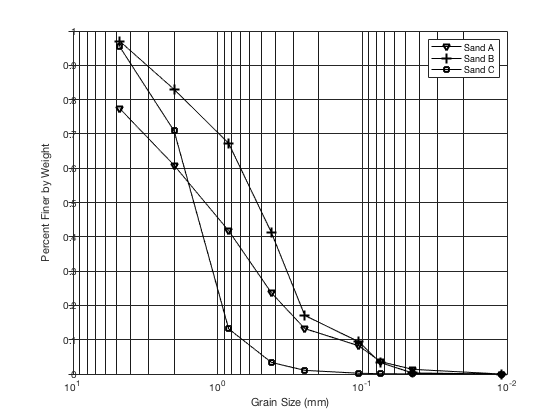
\includegraphics [width=4in]{HomeworkTwo_02.eps}



\end{document}
    
